\begin{frame}{Idea}
	\vspace{-20pt}
	\begin{figure}[htb]
		\centering
		\resizebox{\textwidth}{!}{%
			\begin{tikzpicture}
				\node at (0,0.8) {1 Geometry + 1 Force};
				\node[draw=none, inner sep=0pt] at (0,0) {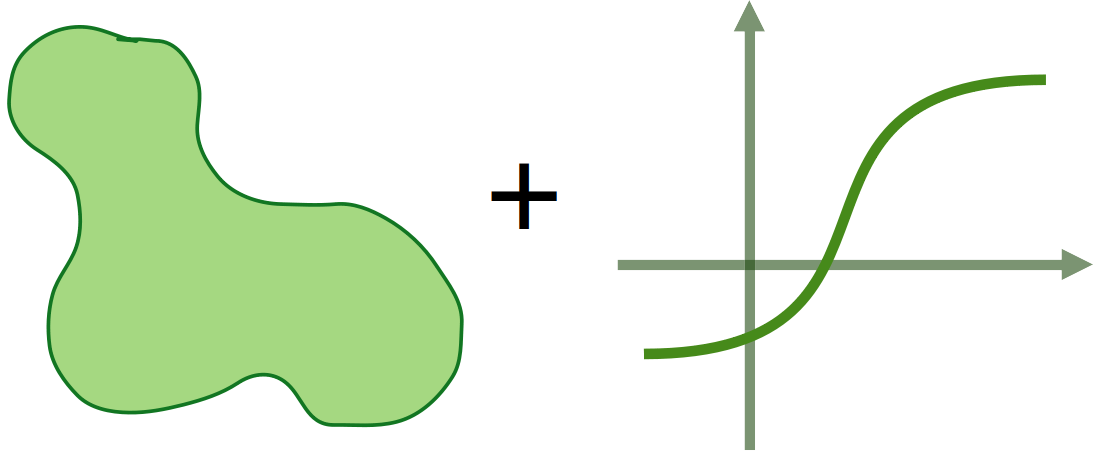
\includegraphics[width=2cm]{images/correction/objective_onegeom_onefct.png}};
				\node at (0,-1) {$\begin{aligned}[t]
						\; \phi \quad \text{\small and} \quad &f \\
						\; (\text{\small and} \quad &g)
					\end{aligned}$};
				
				\draw[->, title, line width=1.5pt] (1.7,0.1) -- (2.7,0.1);
				
				\node[align=center] at (4,1) {Get PINNs prediction};
				\node[draw=none, inner sep=0pt] at (4,0.1) {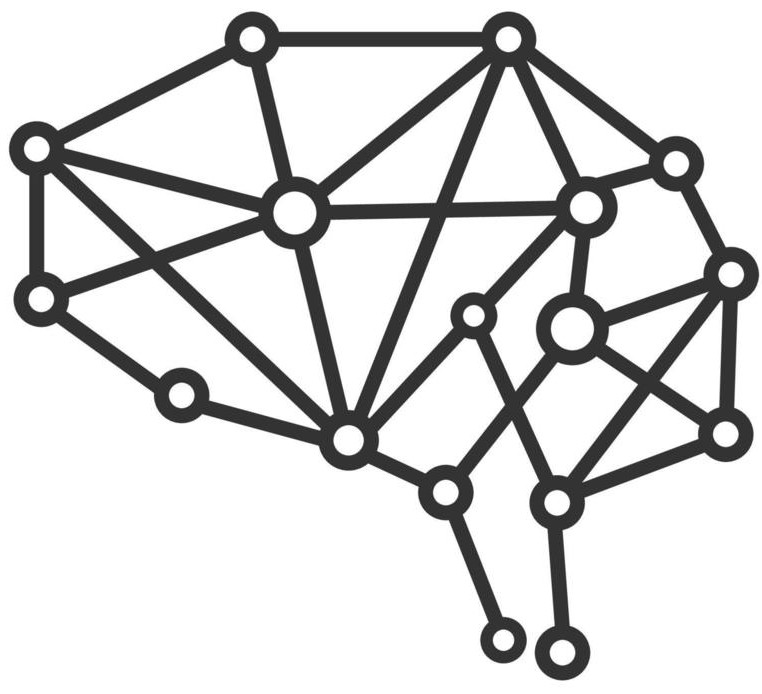
\includegraphics[width=1.4cm]{images/correction/objective_pinns.jpg}};
				\node at (4,-0.8) {\fcolorbox{blue}{white}{$u_{NN}=\phi w_{NN}+g$}};
				\node at (4,-1.3) {\textcolor{blue}{$u_{NN}=g$ on $\Gamma$}};
				
				% Ajouter une flèche entre les deux rectangles
				\draw[->, title, line width=1.5pt] (5.2,0.1) -- (6.2,0.1);
				
				\node[align=center] at (7.8,1) {Correct prediction \\ with FEM};
				\node[draw=none, inner sep=0pt] at (7.8,-0.1) {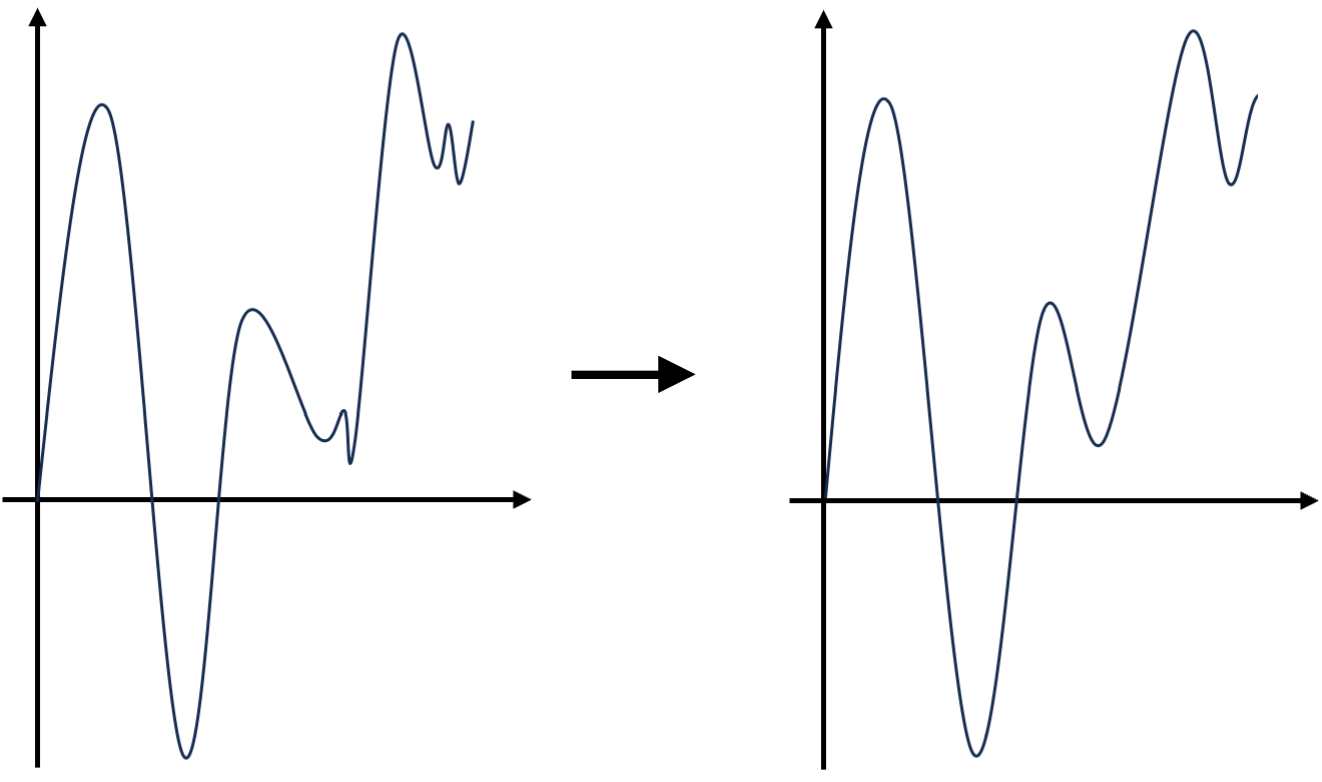
\includegraphics[width=2.5cm]{images/correction/objective_corr.png}};		
				\node at (7.8,-1) {$u_{NN}\rightarrow\tilde{u}=u_{NN}+\tilde{C}$};
			\end{tikzpicture} 
		}%
	\end{figure}
	
	\vspace{-5pt}
	
	\textbf{Correct by adding :} Considering $u_{NN}$ as the prediction of our PINNs for (\ref{edp}), the correction problem consists in writing the solution as
	\begin{equation*}
		\tilde{u}=u_{NN}+\underset{\textcolor{red}{\ll 1}}{\fcolorbox{red}{white}{$\tilde{C}$}}
	\end{equation*}
	
	\vspace{-8pt}
	\begin{minipage}{\linewidth}
		\setstretch{0.5}
		and searching $\tilde{C}: \Omega \rightarrow \mathbb{R}^d$ such that
		\begin{equation*}
			\left\{\begin{aligned}
				L(\tilde{C})&=\tilde{f}, \; &&\text{in } \Omega, \\
				\tilde{C}&=0, \; &&\text{on } \Gamma,
			\end{aligned}\right. %\tag{$\mathcal{C}_{+}$} %\label{corr_add}
		\end{equation*}
		with $\tilde{f}=f-L(u_{NN})$. \refappendix{frame:fem}
	\end{minipage}
\end{frame}

\begin{frame}{Poisson on Square}
	Solving the \textcolor{orange}{Poisson problem} with homogeneous Dirichlet BC. \\
	\ding{217} \textbf{Domain :} $\Omega=[−0.5\pi,0.5\pi]^2$ \\
	\ding{217} \textbf{Analytical levelset function :}
	\small
	\begin{equation*}
		\phi(x,y)=(x-0.5\pi)(x+0.5\pi)(y-0.5\pi)(y+0.5\pi)
	\end{equation*} 
	\ding{217} \textbf{Analytical solution :}
	\small
	
	\vspace{-8pt}
	\begin{equation*}
		u_{ex}(x,y)=\exp\left(−\frac{(x-\mu_1)^2+(y-\mu_2)^2}{2}\right)\sin(2x)\sin(2y)
	\end{equation*} 
	\normalsize
	with $\mu_1,\mu_2\in[-0.5,0.5]$. 
	
	\vspace{8pt}
	Taking $\mu_1=0.05,\mu_2=0.22$, the solution is given by
	\begin{minipage}{0.68\linewidth}
		\centering
		\pgfimage[width=\linewidth]{images/correction/poisson_sol.png}
	\end{minipage}
	\begin{minipage}{0.28\linewidth}
		\flushright
		\pgfimage[width=0.9\linewidth]{images/correction/poisson_loss.png}
	\end{minipage}
\end{frame}

\begin{frame}{Theoretical results}
	TODO
	$\mu_1=0.05,\mu_2=0.22$
	\begin{center}
		\pgfimage[width=0.5\linewidth]{images/correction/theoretical.png}
	\end{center}
\end{frame}

\begin{frame}{Gains using our approach}	
	\vspace{10pt}
	
	\hspace{20pt}\begin{minipage}{0.05\linewidth}
		\footnotesize
		\rotatebox[origin=b]{90}{\textbf{Solution $\mathbb{P}_1$}} 
	\end{minipage}
	\begin{minipage}{0.8\linewidth}
		\centering
		\pgfimage[height=1.7cm]{images/correction/gains_P1.png}
	\end{minipage} 

	\vspace{5pt}

	\hspace{20pt}\begin{minipage}{0.05\linewidth}
		\footnotesize
		\rotatebox[origin=b]{90}{\textbf{Solution $\mathbb{P}_2$}} 
	\end{minipage}
	\begin{minipage}{0.8\linewidth}
		\centering
		\pgfimage[height=1.7cm]{images/correction/gains_P2.png}
	\end{minipage} 

	\vspace{5pt}

	\hspace{20pt}\begin{minipage}{0.05\linewidth}
		\footnotesize
		\rotatebox[origin=b]{90}{\textbf{Solution $\mathbb{P}_3$}} 
	\end{minipage}
	\begin{minipage}{0.8\linewidth}
		\centering
		\pgfimage[height=1.7cm]{images/correction/gains_P3.png}
	\end{minipage} 
\end{frame}

\begin{frame}{Time/Precision}	
	TODO
\end{frame}
